\begin{figure}[h]
  \centering
  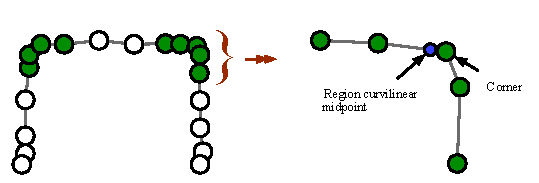
\includegraphics[width=0.8\linewidth]{img/clusters-curvature.pdf}
  \caption[Curvature clusters and corners]{Corner finding begins by
    clustering nearby points that have high curvature. At left, the
    stroke has two such clusters indicated with dark circles. At
    right, one cluster is shown up close. The cluster's curvilinear
    midpoint is found, and the point nearest that midpoint becomes the
    corner.}
  \label{fig:corner-finding}
\end{figure}
